\section {Interactions}
\label{sec:related_work_interactions}

Interactions are a crucial tool to improve data quality of the point cloud. Tasks like removing unwanted points, selecting regions of interest, or creating new geometry are examples of interactions that can be performed on point clouds to create more distinct visual representations of the objects in the point cloud. Many tasks require a selection of points of interest beforehand. 

\par

The lasso interaction is a common tool to select regions in two-dimensional screen space. Lucas et al. \cite{lucas2005design} brought the lasso interaction into a tree-dimensional environment by drawing the lasso on a tracked 2D canvas that shows a desired view of the scene. Elmqvist et al. \cite{elmqvist2008rolling} propose to perform a selection in multi-dimensional data by selecting data sequentially in different 2D scatterplots using the lasso selection. 

\par

Yu et al. \cite{yu2012efficient} present two new methods of interaction using only two-dimensional input. The results are two techniques that turn a two-dimensional lasso into a three-dimensional volume that is fitted to the spatial structure of the point cloud. Similar to sketch-based modeling \cite{igarashi2007teddy}, TeddySelection inflates a user-drawn lasso using a heuristic that takes the local point density into account and fits it to the indented region. CloudLasso uses the Marching Cubes algorithm \cite{lorensen1987marching} to identify and select regions within the lasso where the density is beyond a threshold. Both techniques only use two degrees of freedom, thus can be used in a traditional mouse-based interaction, as well as in direct-touch environments. 

\begin{figure}[ht]
    \centering
    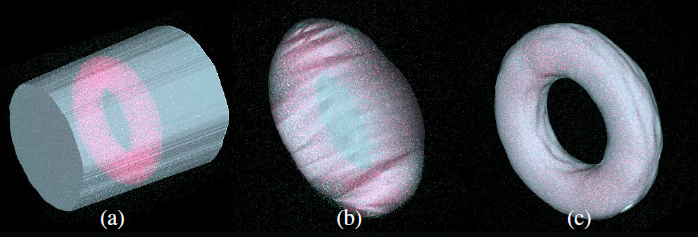
\includegraphics[width=0.81\textwidth]{Related_Work/teddyCloudSelection.png}%7
    \caption[Comparison of (a) simple lasso selection, (b) TeddySelection and (c) CloudLasso]
		{The region in grey describes the selection volume. Points that are selected are colored in pink. (a) shows a classic lasso selection, (b) shows a TeddySelection and (c) shows the CloudLasso. Image by Yu et al.\cite{yu2012efficient}.}
    \label{fig:teddyCloudSelection}
\end{figure}

Figure \ref{fig:teddyCloudSelection} compares the results of a simple lasso selection, TeddySelection and the CloudLasso. 

\par

An example of a three-dimensional interaction technique is the Volumetric Brush by Weyrich et al. \cite{weyrich2004post}. The brush follows the local curvature by retrieving the current depth value for the cursor's position from the z-Buffer. The reconstructed world-space position is then used to as the center of a volume, usually a sphere, to select points. Scheiblauer and Wimmer \cite{scheiblauer2011out} utilize the volumetric brush for selections in point clouds. 

\par

Picking is a special case of selection where only a single element is selected. Raycasting is used frequently due to its simplicity for the user and performance over distance. However, raycasting on large datasets is limited by the CPU quickly as extensive geometric intersections must be calculated for each object. 

\par

Zhu et al. \cite{zhu2008algorithm} present a picking technique for 3-dimensional objects based on view space. The authors propose the use of a bounding-box tree. This hierarchical structure makes it easy to perform view culling and prematurely discard objects that do not intersect the pick ray. The bounding boxes are transformed into view space, where a first intersection is calculated. If a box intersects, intersections with the actual object are calculated. 
Zhang et al. \cite{zhang20093d} propose two GPU-driven primitive-picking algorithms. The first method renders the primitives along with a unique id into a render target texture and retrieves the pick information by downloading the texture. The second approach performs the pick ray intersections in screen space by transforming each primitive using a geometry shader that emits the intersection information. The CPU retrieves this information using transform feedback.

\par

Huang et al. \cite{huang2014pickup} propose a GPU-driven implementation for point picking in large-scale point clouds. The idea is to perform picking in screen space and choose the point that is closest to the mouse position. Their approach utilizes the parallel architecture of the graphics card for screen-space transformations and distance measures for all points. Potree \cite{SCHUETZ-2016-POT} applies a similar technique without the use of compute shaders. Instead, a unique per-point id is rendered into a texture from which a small window around the cursor is downloaded to the CPU, and the final picking decision is performed.  